\subsubsection{Design af elementer}
Herunder vil designet af en stor del af Kommunikationen i grænsefladen blive beskrevet, både med klassediagrammer og sekvensdiagrammer.\\

\textbf{Klassediagrammer}\\

\begin{figure}[H]
	\centering
	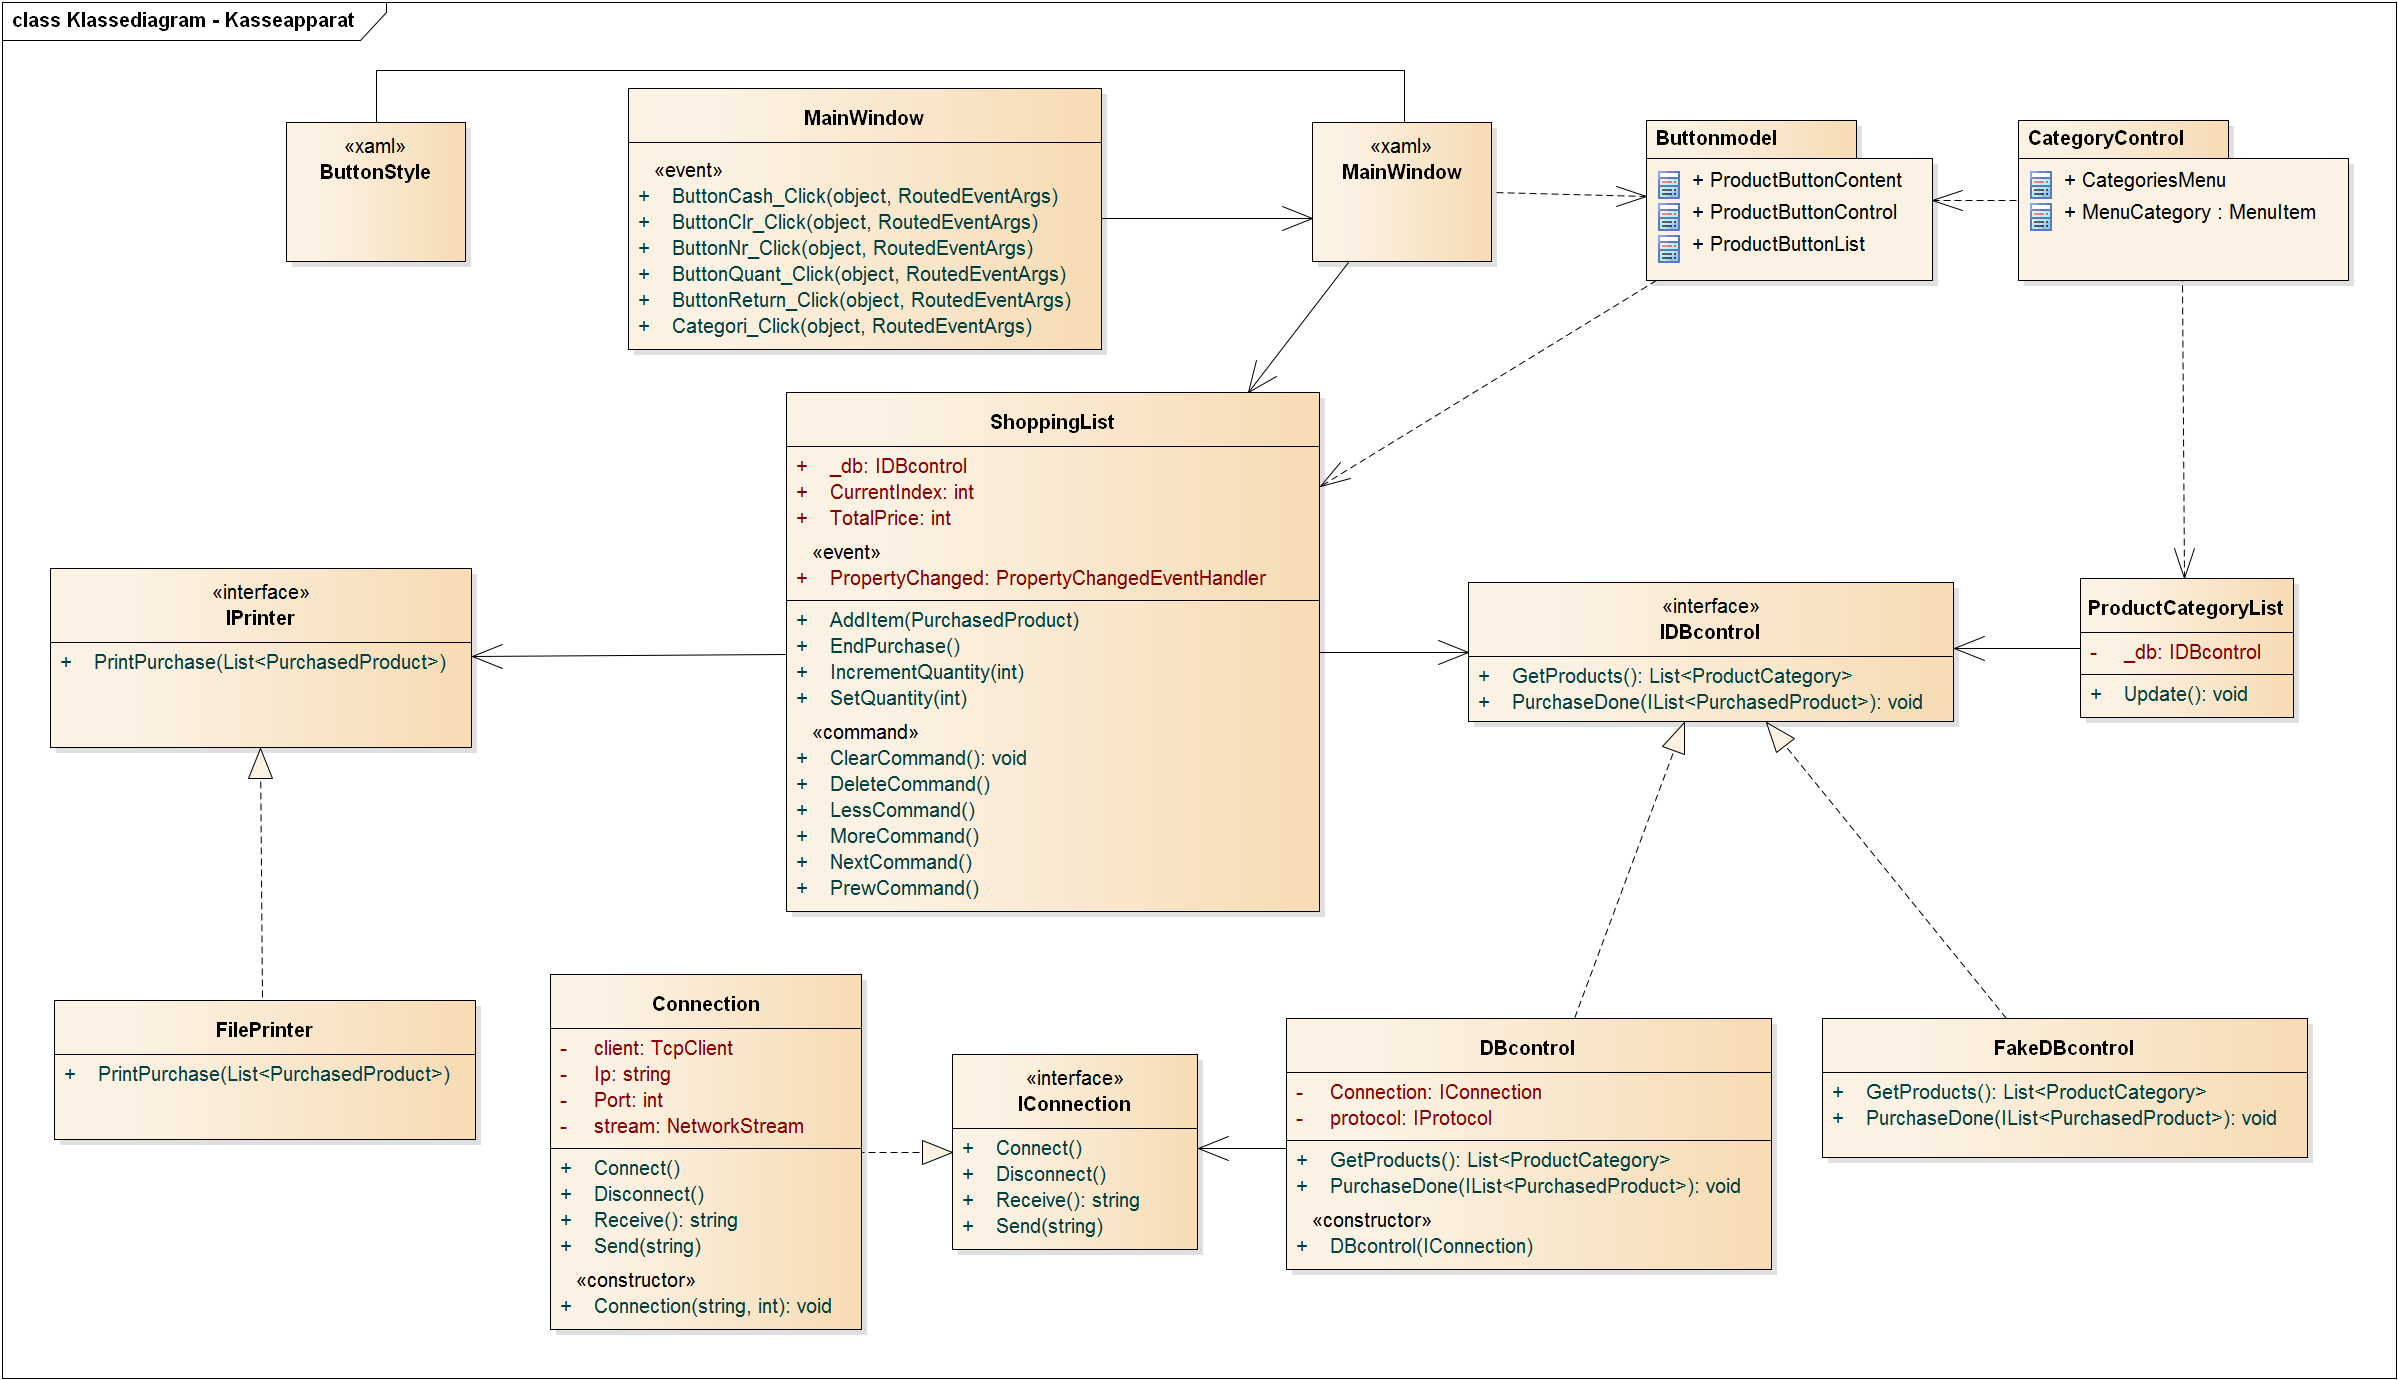
\includegraphics[width=1.2\textwidth, angle=90]{Systemdesign/Frontend/GUI/DesignOgStruktur/Pics/KlassediagramKasseApparat}
	\caption{Klassediagram over kasseapparat.}
	\label{fig:KasseKlasse}
\end{figure}

På figur \ref{fig:KasseKlasse} kan man se hele kasseapparatets software vist ved dens klasser og funktioner. Dog er ViewModels delt op i 2 pakker. Dette er bestemt, da det ville give mere mening at gøre det på denne måde, når man skulle forklare klasserne og deres indbyrdes forhold. Disse forhold vil blive nærmere beskrevet ved figur \ref{fig:ButtonModel} og \ref{fig:CategoryControl} \\
Klassediagrammet er delt op i 3 lag, der skal symbolisere henholdsvis Presentation-, Business Logic- og Data Access Layer.

\begin{figure}[H]
	\centering
	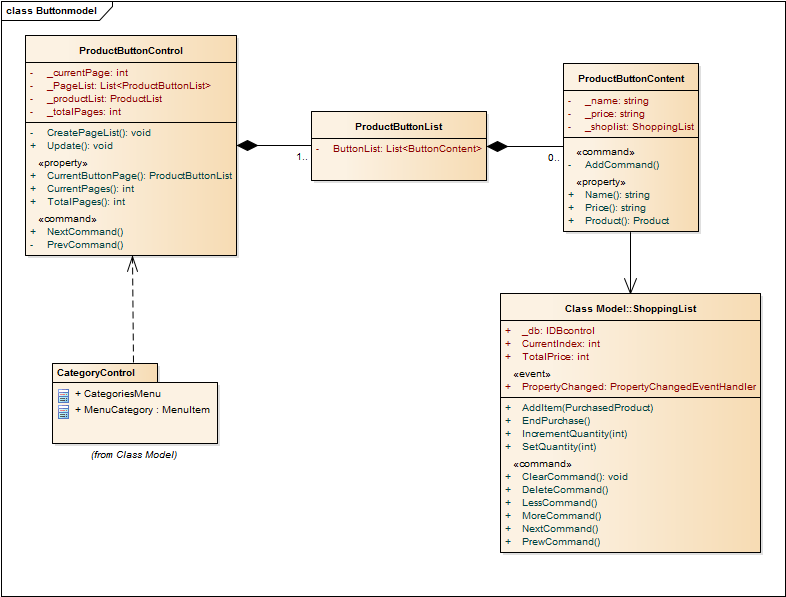
\includegraphics[width=0.7\textwidth]{Systemdesign/Frontend/GUI/DesignOgStruktur/Pics/KlassediagramButtonModel}
	\caption{Klassediagram over ViewModel pakken ButtonModel.}
	\label{fig:ButtonModel}
\end{figure}

På figur \ref{fig:ButtonModel} ser man ViewModel pakken buttonmodel, der står for produktknapperne i grænsefladen. Disse objekter sikrer at man kan skifte produktside og ved tryk på en knap kan et produkt tilføjes til shoppinglist som er indkøbskurven på \gls{KA}tet. For at opsætte denne pakke blev der først opsat et sekvensdiagram set på figur.

\begin{figure}[H]
	\centering
	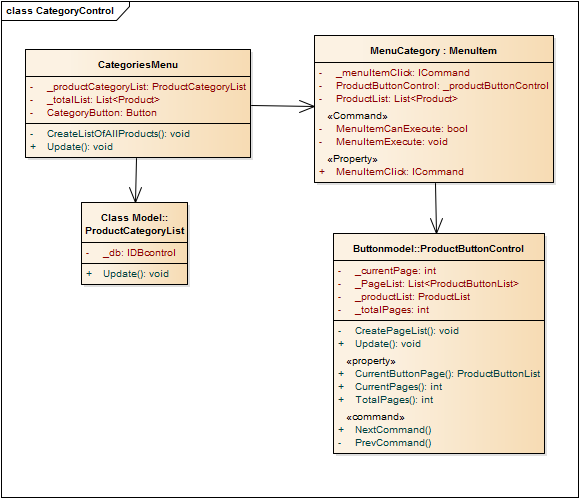
\includegraphics[width=0.7\textwidth]{Systemdesign/Frontend/GUI/DesignOgStruktur/Pics/KlassediagramCategoryControl}
	\caption{Pakkediagram over ViewModel pakken CategoryControl.}
	\label{fig:CategoryControl}
\end{figure}

CategoryControl er en ViewModel pakke der står for at kontrollere produktkategori valg og dermed hvilke produkter der vises i grænsefladen. Denne ViewModel pakke kender til ProductButtonControl, da den derved kan oprette de ønskede produktknapper ved tryk på en kategori. Viden om eksisterende kategorier får pakken ved ProductCategoryList. \\

\textbf{Sekvensdiagrammer} \\
For at forstå kommunikationen mellem de forskellige klasser/ pakker er de følgende sekvensdiagrammer blevet opsat. \\

\begin{figure}[H]
	\centering
	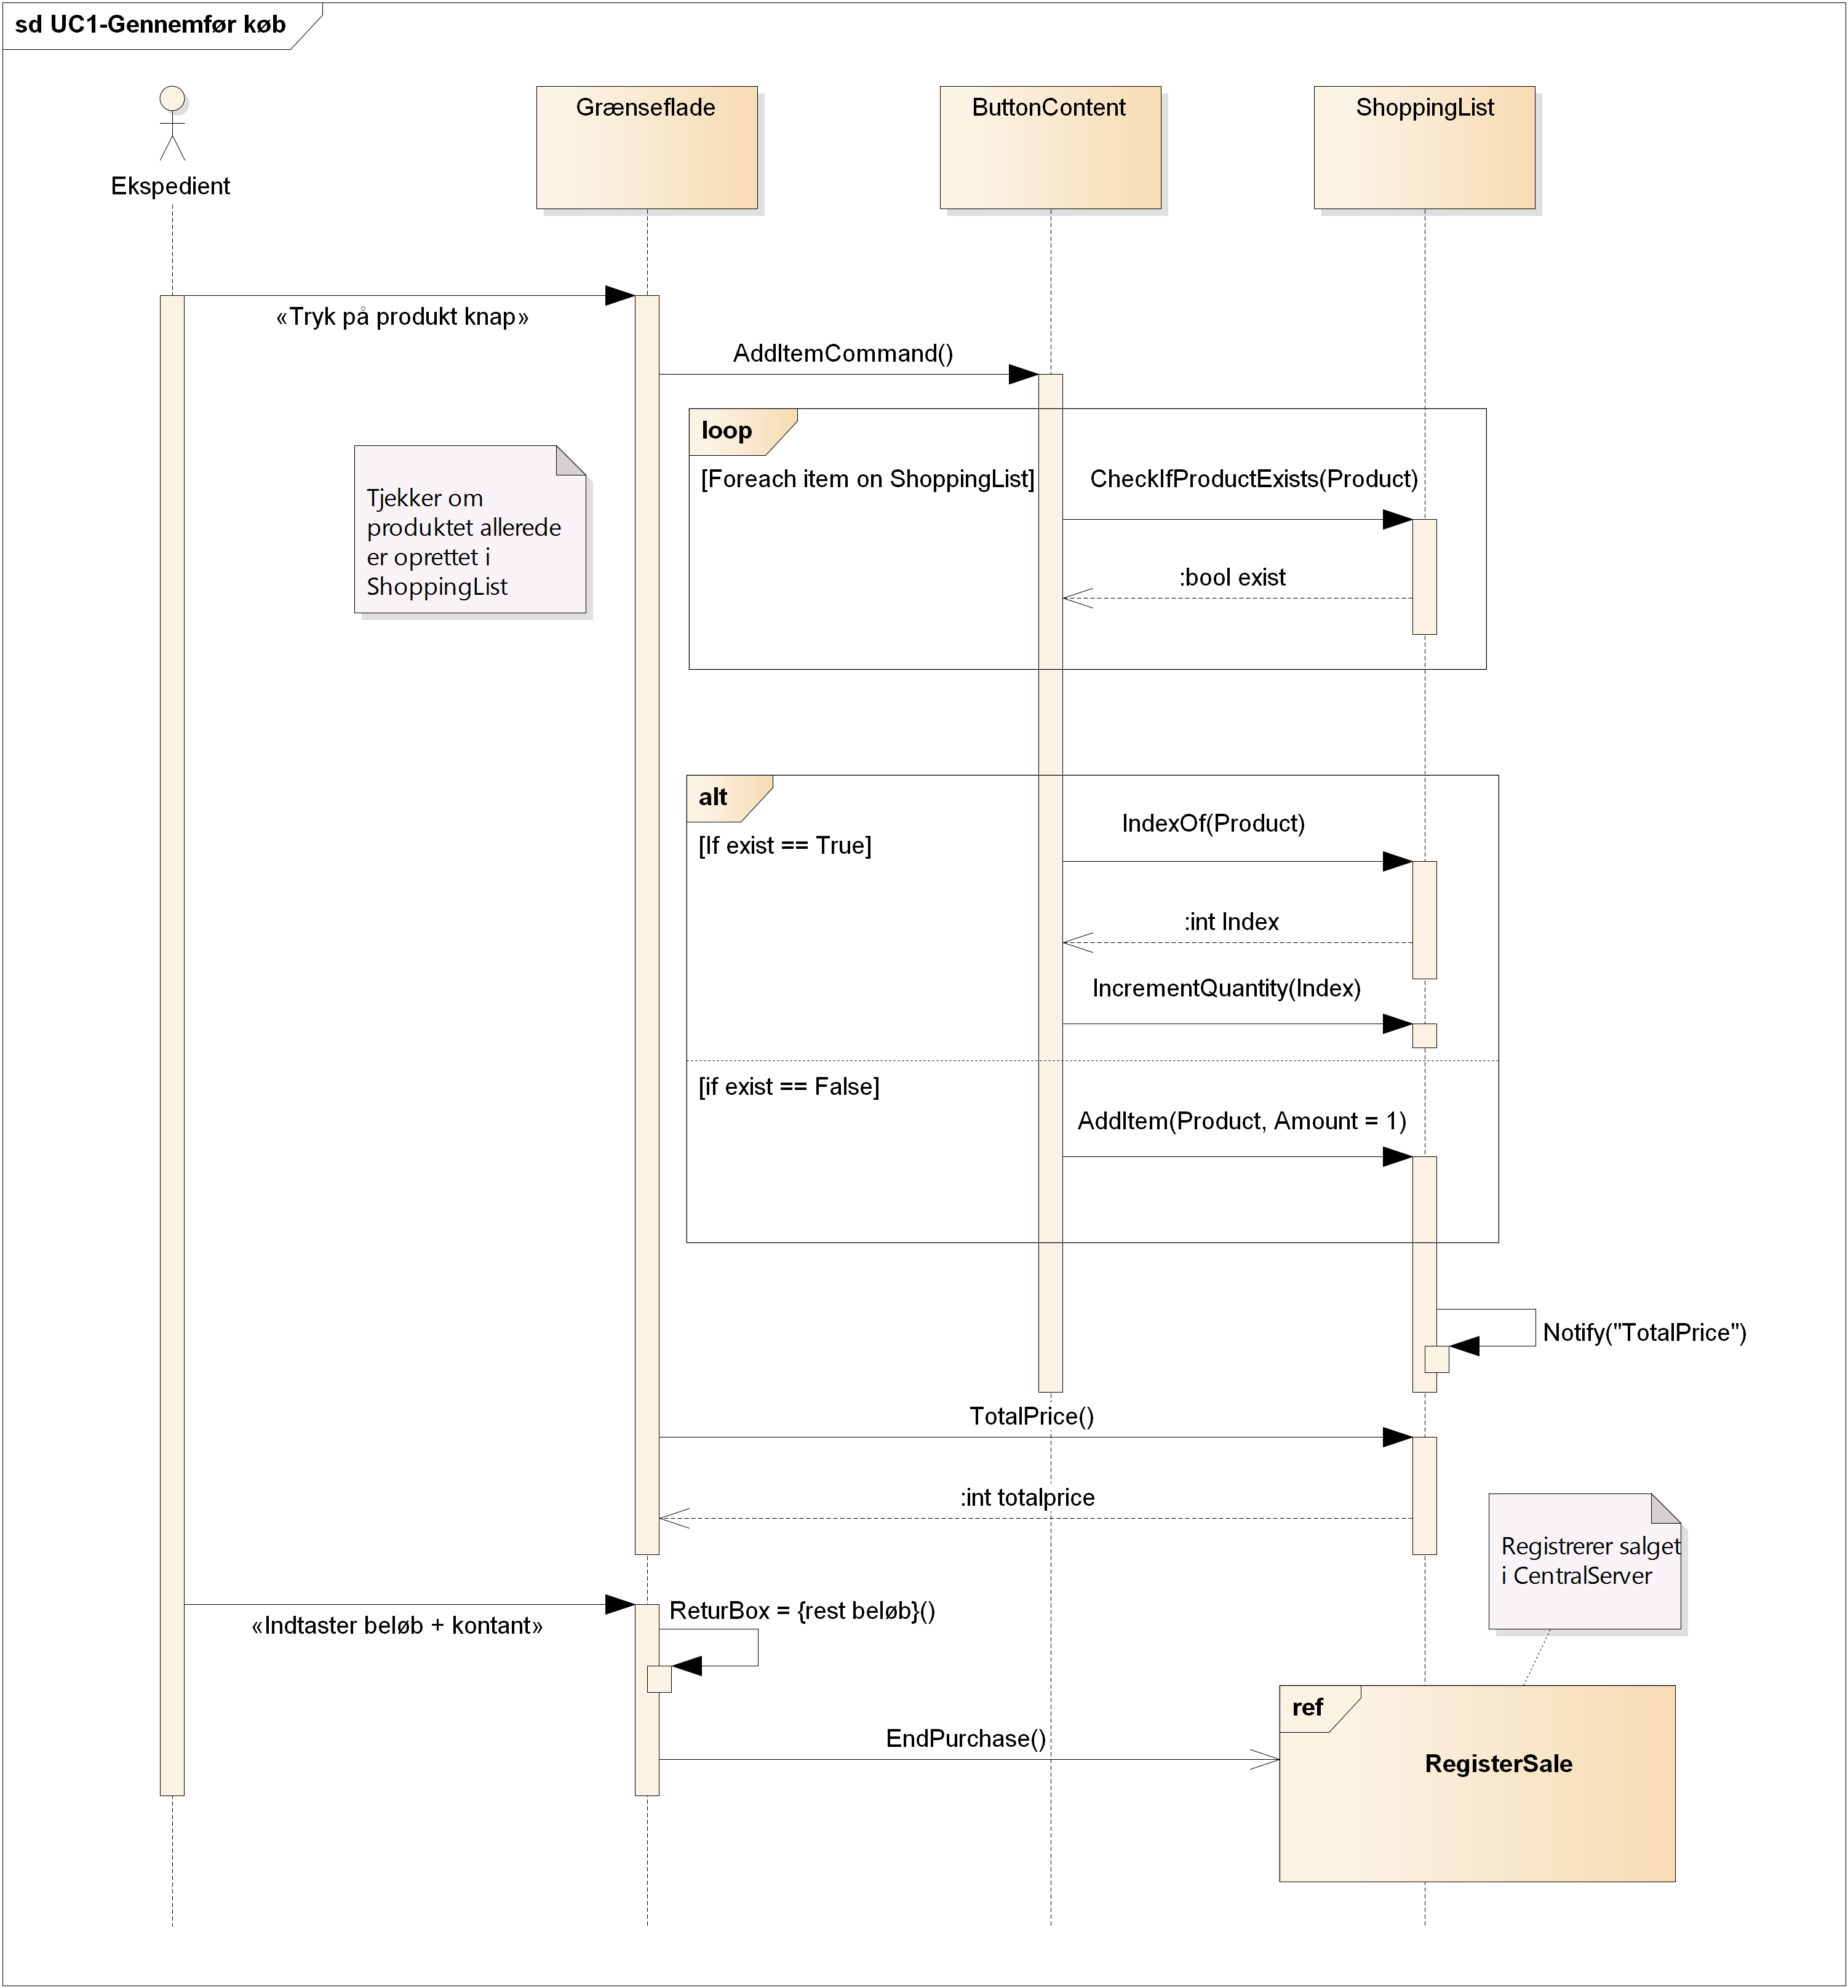
\includegraphics[width=1\textwidth]{Systemdesign/Frontend/GUI/Pics/Sekvensdiagram-TilfoejProdukt2}
	\caption{Sekvensdiagram over tilføjelse af produkt til shoppinglist}
	\label{fig:SekvensUC1}
\end{figure}

På figur \ref{fig:SekvensUC1} er der opsat et sekvensdiagram over Use Case 1 - Gennemfør køb. Her kan man se hvad der sker når en ekspedient starter et salg ved at vælge et produkt i grænsefladen. Når knappen bliver trykket ned, så kalder viewet AddItemCommand i ViewModellen ButtonContent. Dette command tjekker så om der allerede er tilføjet et produkt i shoppinglist. Hvis der er, inkrementeres produktet. Hvis ikke så tilføjes det. Herefter notifier shoppinglist på at der er ændret på totalprice og denne nye værdi hentes derefter af viewet. \\
Nu da produktet er tilføjet til shoppinglist kan ekspedienten tage imod penge fra kunden, trykke beløbet ind og så til sidst trykke på kontant. Herefter bliver salget så registreret i CentralServeren og der bliver lavet en kvittering ved et kald i FilePrinter.

\begin{figure}[H]
	\centering
	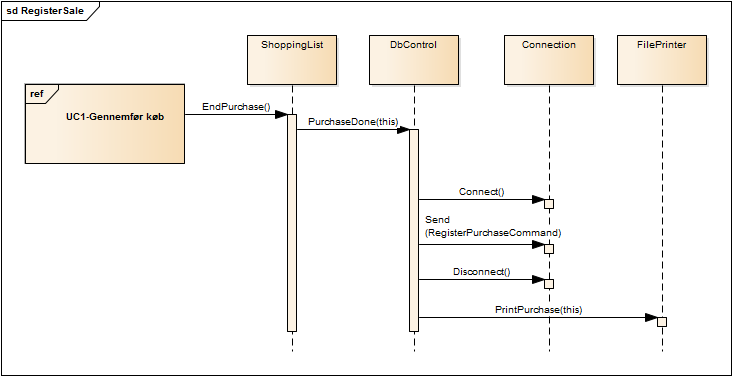
\includegraphics[width=1\textwidth]{Systemdesign/Frontend/GUI/DesignOgStruktur/Pics/RegisterSale}
	\caption{Sekvensdiagram over opstart system}
	\label{fig:SekvensOpstart}
\end{figure}

\begin{figure}[H]
	\centering
	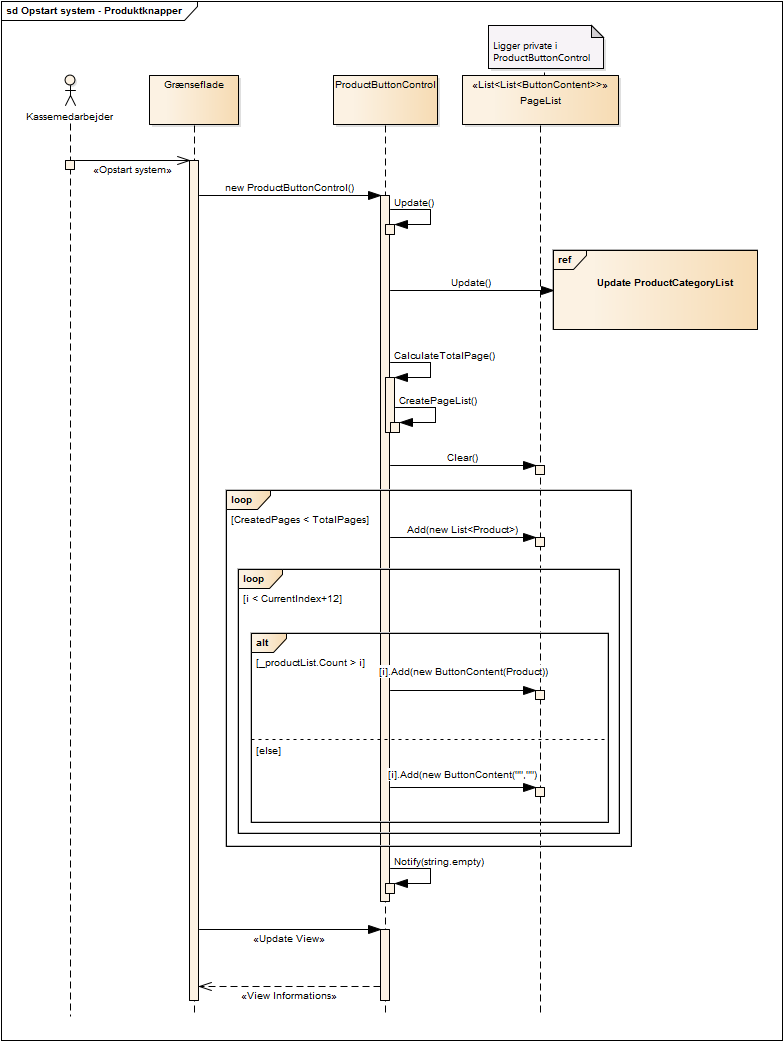
\includegraphics[width=1\textwidth]{Systemdesign/Frontend/GUI/DesignOgStruktur/Pics/OpstartSystem}
	\caption{Sekvensdiagram over opstart system}
	\label{fig:SekvensOpstart}
\end{figure}

stuff to be written

\begin{figure}[H]
	\centering
	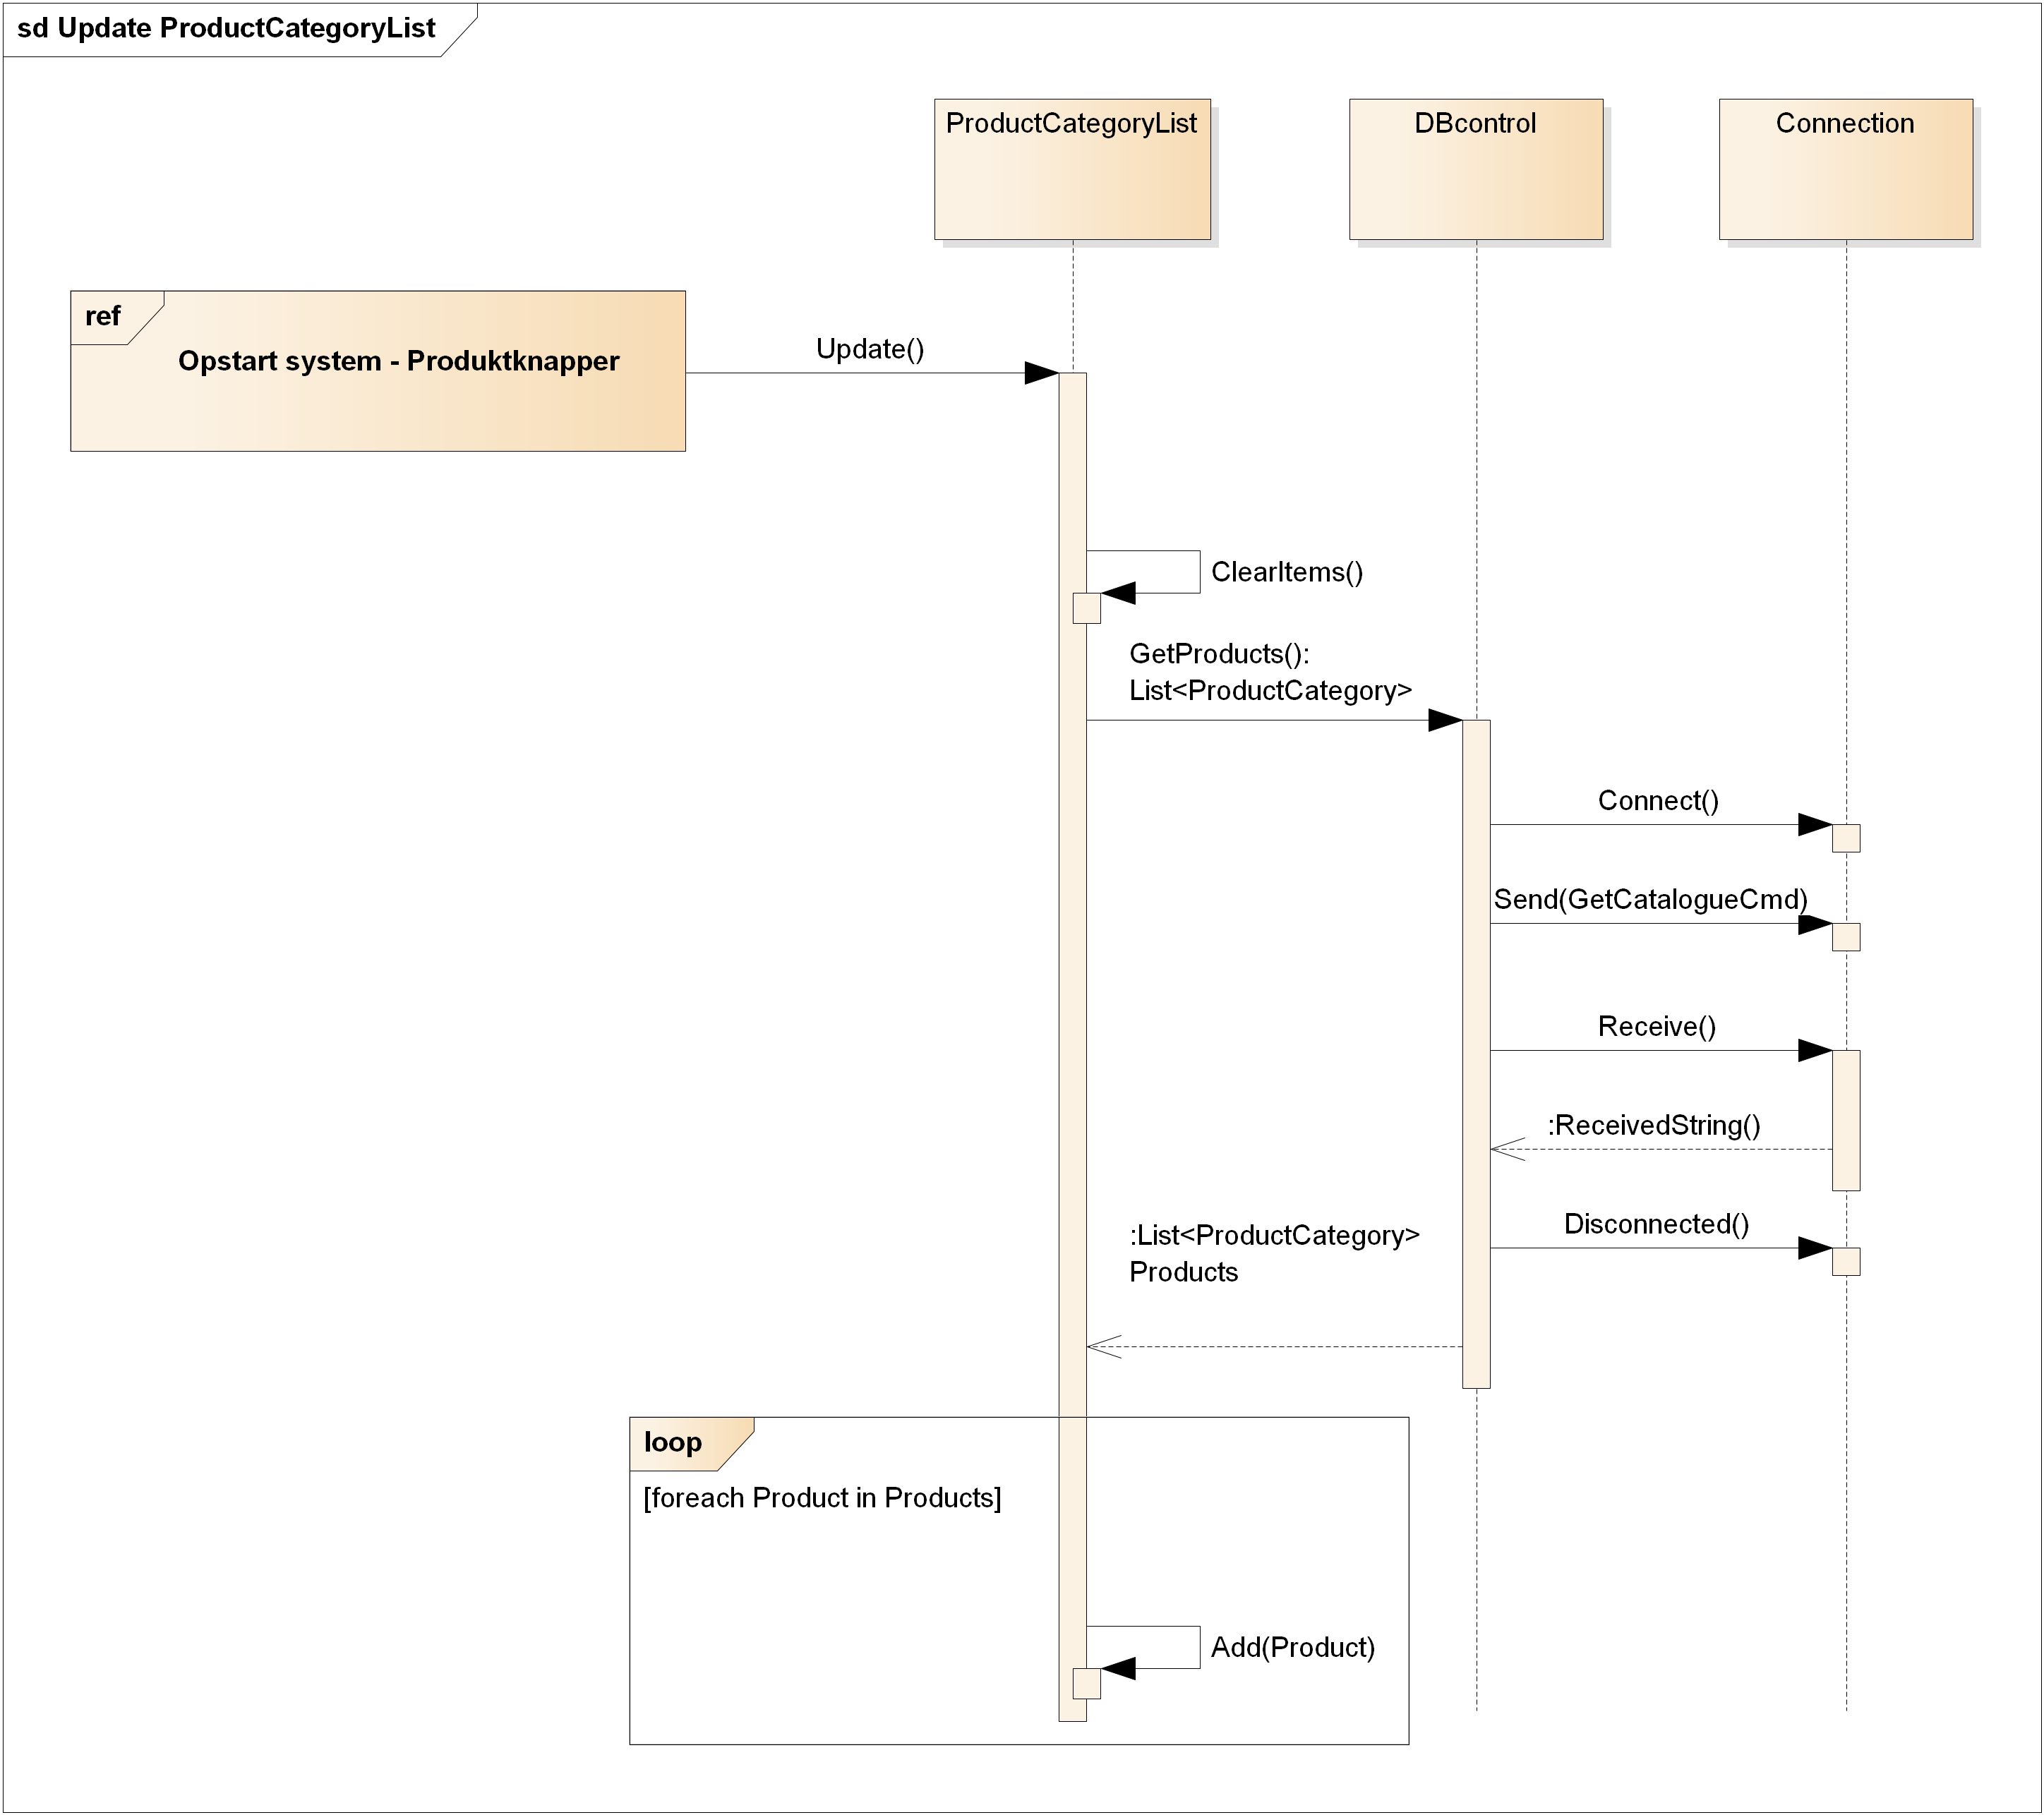
\includegraphics[width=1\textwidth]{Systemdesign/Frontend/GUI/DesignOgStruktur/Pics/UpdateProductCategoryList}
	\caption{Sekvensdiagram over Update System}
	\label{fig:SekvensUpdate}
\end{figure}

More stuff to be written

\newpage
